
\documentclass[11pt]{article}

\usepackage[margin=1in]{geometry}
\usepackage{amsmath,amssymb,amsfonts}
\usepackage{booktabs}
\usepackage{graphicx}
\usepackage{natbib}
\usepackage{hyperref}
\usepackage{enumitem}
\usepackage{array}
\usepackage{caption}

\hypersetup{
    colorlinks=true,
    linkcolor=blue,
    citecolor=blue,
    urlcolor=blue
}

\newcommand{\R}{\mathbb{R}}
\newcommand{\argmax}{\operatorname*{arg\,max}}

\title{Dynamic Prediction-Decision Learning for Portfolio Optimization:\\
A Preliminary Study with Seven Exchange-Traded Funds}

\author{
Tiantian ZHANG\\
Columbia University\\
Work initiated during an internship at Boke Simu\\
\texttt{t.zhang8@columbia.edu}\\
\texttt{tiantianzhang02@bokesimu.com}
}

\date{Preliminary draft, April 2026}

\begin{document}

\maketitle

\begin{abstract}
Modern portfolio optimization is often implemented as a static or myopic procedure: a predictor estimates returns or risk, and a downstream optimizer converts these estimates into portfolio weights. Recent integrated prediction-optimization methods attempt to close this mismatch by differentiating through the optimizer and training the predictor directly against portfolio performance. This paper studies whether such integration is necessary, or whether a more modular architecture can capture dynamic trading objectives more effectively. We propose a prediction-decision framework in which a deep temporal prediction layer extracts market state and future-return information, while a reinforcement-learning decision layer learns state-dependent portfolio actions under transaction cost, risk, and no-trade constraints. The decision layer is formulated through a Bellman reward that explicitly includes previous holdings, so that current allocation decisions are evaluated by their effect on future rebalancing value. We compare two-stage learning, integrated learning, finite-action fitted Q iteration, and a preliminary deep conservative Q-learning fitted-Q-iteration proxy on a seven-ETF universe using rolling out-of-sample experiments. The experiments are intentionally preliminary. They show that integrated learning, in the current implementation, is slower and does not outperform the two-stage baseline, while a constrained deep RL decision layer improves over plain fitted Q iteration and the integrated baseline but still fails to beat an equal-weight portfolio in the tested 2019 rolling window. These results suggest that dynamic reward design is central to deep learning for portfolio optimization: the promising direction is not to replace prediction with black-box reinforcement learning, but to combine deep prediction with conservative Bellman decision learning.
\end{abstract}

\paragraph{Keywords.}
Portfolio optimization; dynamic portfolio choice; deep learning; reinforcement learning; fitted Q iteration; conservative Q-learning; transaction costs; prediction-decision learning.

\section{Introduction}

Portfolio allocation is a sequential decision problem. The portfolio held today affects both today's realized return and tomorrow's feasible rebalancing cost. Nevertheless, many empirical machine-learning portfolio pipelines are still organized around a static or two-stage structure: a model predicts future returns, and a separate optimizer constructs weights from these predictions. This separation is simple, stable, and often strong in practice, but it can misalign prediction accuracy with the downstream trading objective. A forecast that minimizes mean-squared error need not produce the best portfolio after risk and transaction costs are included.

Recent work on integrated prediction and multi-period portfolio optimization argues that this separation can be improved by making the optimizer differentiable and training the predictor directly through the portfolio objective \citep{LinghuLiuDeng2025IPMO}. This view is closely related to predict-and-optimize learning and SPO-style decision-aware training \citep{ElmachtoubGrigas2022}. Integrated learning is attractive because, in principle, it directly aligns the prediction layer with the financial decision. However, it is also computationally expensive because an optimization problem is solved, and often differentiated through, at each training step.

This paper takes a complementary view. The central question is not only whether prediction and optimization should be integrated, but how to represent the dynamic nature of portfolio trading. The static optimizer asks ``what allocation is best now?'' A dynamic decision rule asks ``if I change from my current holdings to this allocation, how will that affect future returns, future risk, and future rebalancing costs?'' This suggests a reinforcement-learning or dynamic-programming formulation, but financial data are scarce and noisy relative to the data-rich settings in which large-scale reinforcement learning often succeeds.

We therefore study a modular architecture:
\[
\text{past market data}
\quad\longrightarrow\quad
\text{deep prediction layer}
\quad\longrightarrow\quad
\text{dynamic decision layer}.
\]
The prediction layer learns a representation of past market state and future return/risk information. The decision layer learns a value function over state-action pairs, where the state includes the previous portfolio weight and the action is a candidate allocation. The reward explicitly penalizes transaction costs and risk, so the value function internalizes the future consequences of trading.

The present manuscript is preliminary. It reports diagnostic experiments on seven U.S. ETFs using Wind data accessed through Boke City / Boke Simu during the author's internship. The empirical purpose is not to claim a final trading strategy, but to identify which research direction is most plausible. The main findings are:
\begin{enumerate}[leftmargin=*]
    \item In small rolling tests, integrated prediction-optimization does not outperform two-stage prediction. It is slower, and in our implementation it produces higher turnover.
    \item Plain fitted Q iteration (FQI) is not sufficient: it overtrades and loses much of its gross performance after transaction costs.
    \item A deep conservative FQI proxy with an auxiliary prediction head and a no-trade threshold improves over plain FQI, two-stage, and integrated baselines in the 12-block rolling test, but still does not outperform equal weight.
    \item The strongest lesson is that reward design matters. A useful dynamic learning system must combine prediction, transaction costs, risk control, and conservative policy updates.
\end{enumerate}

\section{Related Work}

\paragraph{Mean-variance and dynamic portfolio choice.}
The classical mean-variance framework of \citet{Markowitz1952} optimizes a risk-return tradeoff at a given investment horizon. In practice, portfolio management is dynamic because current holdings create future transaction costs and because future market regimes change. Dynamic portfolio choice with transaction costs has therefore been studied both in traditional optimization and in learning-based frameworks.

\paragraph{Smart predict-then-optimize and integrated learning.}
Smart predict-then-optimize (SPO) trains predictive models by the decision error induced by their predictions rather than by pointwise forecast error \citep{ElmachtoubGrigas2022}. Integrated prediction and multi-period portfolio optimization (IPMO) extends this motivation to a multi-period mean-variance portfolio problem with turnover penalties, using a differentiable optimization layer and mirror-descent fixed-point differentiation for scalability \citep{LinghuLiuDeng2025IPMO}. In contrast to SPO-style regret surrogates, the integrated portfolio architecture differentiates through a continuous constrained optimizer and uses realized portfolio utility as the training signal.

\paragraph{Deep reinforcement learning for portfolios.}
Reinforcement learning naturally models sequential portfolio trading through a Markov decision process (MDP). Recent work by \citet{JiangOlmoAtwi2024} proposes a TD3-based deep reinforcement-learning framework for portfolio selection that embeds investor risk aversion and transaction costs in an extended mean-variance reward. Their model is evaluated on DJIA and S\&P100 constituents and shows that transaction-cost and risk-aware reward design is essential. This paper borrows the MDP and reward-design perspective, but begins with a simpler finite-action offline-RL proxy because the present ETF universe is small and the rolling training sample is limited.

\paragraph{Offline RL and conservative Q-learning.}
Fitted Q iteration (FQI) is a batch-mode reinforcement-learning algorithm that repeatedly fits a supervised model to Bellman targets \citep{ErnstGeurtsWehenkel2005}. It is suitable as a first proxy for financial data because the training data are offline historical trajectories rather than interactions with a simulator. A key risk in offline RL is value overestimation for actions not well covered by the historical data. Conservative Q-learning (CQL) addresses this by penalizing high Q-values on unlikely or out-of-distribution actions \citep{Kumar2020CQL}. Our preliminary deep CQL-FQI proxy follows this idea in a finite candidate-action setting and adds a no-trade threshold to reduce turnover.

\paragraph{Decision-distribution learning and large language models.}
Preference-optimization methods in large language models, such as DPO and reward-guided decision-distribution updates, also frame model outputs as decisions. For example, DDO-RM treats each prompt as a finite decision problem over candidate responses and distills a reward-guided target distribution back into the policy \citep{ZhangZuoWang2026DDORM}. The analogy is useful, but direct transfer is limited: language models are trained with far larger datasets, while financial data are noisy, non-stationary, and expensive to sample. For portfolio optimization, Bellman value learning is more natural than pure preference ranking because actions influence future portfolio states.

\section{Problem Setup}

Let $r_t \in \R^N$ be the vector of daily asset returns and let $w_t \in \Delta^N$ be the portfolio weight vector on the simplex,
\[
\Delta^N = \{w \in \R^N: w_i \geq 0,\; \sum_{i=1}^N w_i = 1\}.
\]
The one-period gross portfolio return is
\[
R^{\mathrm{gross}}_t = w_t^\top r_{t+1}.
\]
If $c>0$ is the proportional transaction-cost coefficient, the net return is
\[
R^{\mathrm{net}}_t
=
w_t^\top r_{t+1}
-
c\|w_t-w_{t-1}\|_1.
\]
A risk-aware dynamic reward can be written as
\[
\mathcal{R}_t(s_t,a_t)
=
w(a_t)^\top r_{t+1}
-
c\|w(a_t)-w_{t-1}\|_1
-
\eta\, w(a_t)^\top \Sigma_t w(a_t),
\]
where $\Sigma_t$ is a covariance estimate, $\eta$ controls risk aversion, $s_t$ is the state, and $a_t$ is an allocation action.

The central dynamic object is the state-action value function
\[
Q^\pi(s_t,a_t)
=
\mathbb{E}_{\pi}
\left[
\sum_{k=0}^{\infty}\gamma^k
\mathcal{R}_{t+k}(s_{t+k},a_{t+k})
\;\middle|\;
s_t,a_t
\right],
\]
which satisfies the Bellman relation
\[
Q(s_t,a_t)
=
\mathcal{R}_t(s_t,a_t)
+
\gamma \max_{a'} Q(s_{t+1},a').
\]
This formulation differs from a static optimizer because the previous portfolio $w_{t-1}$ is part of the state and the current action $w_t$ becomes part of the next state.

\section{Prediction-Decision Framework}

\subsection{Prediction Layer}

The prediction layer maps an input window of market information to a latent state and future estimates:
\[
z_t = f_\theta(X_{t-L:t}), \qquad
\hat{\mu}_{t+1:t+H} = g_\theta(z_t).
\]
In the preliminary implementation, $X_{t-L:t}$ contains past ETF returns and the auxiliary prediction head forecasts future returns. The prediction loss is
\[
\mathcal{L}_{\mathrm{pred}}
=
\|\hat{\mu}_{t+1:t+H} - r_{t+1:t+H}\|_2^2.
\]
This supervised head is retained even when a reinforcement-learning decision head is used, because financial rewards are noisy and sparse. The auxiliary prediction objective stabilizes representation learning.

\subsection{Decision Layer}

The decision layer receives $(z_t,w_{t-1})$ and evaluates a finite candidate action set $\mathcal{A}$:
\[
Q_\psi(s_t,a), \qquad a \in \mathcal{A}.
\]
The candidate actions include equal weight, inverse-volatility portfolios, bond-heavy, equity-heavy, gold-heavy, commodity-heavy, momentum portfolios, and a hold/no-trade action. This discretization is intentionally conservative. It avoids the instability of continuous-action actor-critic methods in small samples and makes turnover behavior interpretable.

\subsection{Deep Conservative FQI Objective}

For a transition $(s_t,a_t,R_t,s_{t+1})$, the Bellman target is
\[
y_t
=
R_t
+
\gamma \max_{a'\in\mathcal{A}} Q_{\bar{\psi}}(s_{t+1},a'),
\]
and the fitted-Q loss is
\[
\mathcal{L}_{Q}
=
\left(Q_{\psi}(s_t,a_t)-y_t\right)^2.
\]
We add a conservative penalty that discourages excessively high Q-values for active actions relative to the no-trade action:
\[
\mathcal{L}_{\mathrm{CQL}}
=
\log\sum_{a\in\mathcal{A}}\exp Q_\psi(s_t,a)
-
Q_\psi(s_t,a_{\mathrm{hold}}).
\]
The full training objective is
\[
\mathcal{L}
=
\mathcal{L}_Q
+
\lambda_{\mathrm{pred}}\mathcal{L}_{\mathrm{pred}}
+
\alpha\mathcal{L}_{\mathrm{CQL}}.
\]
At evaluation time, we use a switch threshold:
\[
a_t =
\begin{cases}
\argmax_a Q(s_t,a), & 
Q(s_t,a^*) - Q(s_t,a_{\mathrm{hold}}) > \kappa, \\
a_{\mathrm{hold}}, & \text{otherwise}.
\end{cases}
\]
This threshold is a simple no-trade constraint. It directly targets the overtrading problem observed in preliminary rolling experiments.

\section{Experimental Design}

\subsection{Data}

The empirical study uses seven broad U.S. ETFs:
\[
\{\text{AGG.P},\text{DBC.P},\text{GLD.P},\text{IWM.P},\text{LQD.P},\text{MUB.P},\text{VTI.P}\}.
\]
The raw ETF prices are aligned on common trading dates. The aligned panel contains 4,462 common price dates from 2007-09-10 to 2026-02-06. For the paper-style experiments, we focus on the 2011--2024 period and start the out-of-sample rolling tests at 2019-01-02.

The data source is Wind data accessed through Boke City / Boke Simu during the author's internship. The raw data are not redistributed in this preliminary paper. Public replication would require either permission to use the same data or replacement with a public data source.

\subsection{Rolling Setup}

The rolling setup follows the spirit of the ETF experiments in integrated multi-period portfolio optimization:
\begin{itemize}[leftmargin=*]
    \item training lookback: 250 trading days;
    \item prediction input window: 120 days;
    \item covariance window: 20 days;
    \item test block: 20 daily decisions per roll;
    \item preliminary comparison: 12 rolling blocks, 240 daily out-of-sample decisions;
    \item transaction cost: 20 basis points times daily $\ell_1$ turnover;
    \item evaluation metrics: net NAV, annualized net Sharpe, gross Sharpe, maximum drawdown, and average turnover.
\end{itemize}

\subsection{Baselines}

We compare:
\begin{enumerate}[leftmargin=*]
    \item Equal weight.
    \item Two-stage prediction plus downstream optimization.
    \item Integrated prediction-optimization using a differentiable optimizer layer.
    \item Plain FQI with ridge regression.
    \item Deep CQL-FQI with auxiliary prediction head and no-trade threshold.
\end{enumerate}

The integrated and two-stage baselines are evaluated with the same rolling structure. In the codebase used for this study, the two-stage branch trains the predictor with mean-squared error and optimizes portfolios during validation/testing, while the integrated branch calls the optimizer inside the training loop and optimizes a portfolio return/risk loss.

\section{Preliminary Results}

\subsection{Integrated Versus Two-Stage}

Table~\ref{tab:integrated_two_stage} reports the scaled 12-roll comparison between integrated learning and two-stage learning. Contrary to the integrated-learning hypothesis, the integrated implementation does not outperform two-stage in this diagnostic test. It also has higher turnover and substantially higher runtime.

\begin{table}[htbp]
\centering
\caption{Integrated versus two-stage learning in the 12-roll preliminary setting.}
\label{tab:integrated_two_stage}
\begin{tabular}{lrrrrr}
\toprule
Configuration & Two-stage Sharpe & Integrated Sharpe & Two-stage NAV & Integrated NAV & Runtime Ratio \\
\midrule
$H=10$ & 1.477 & 1.145 & 1.074 & 1.057 & 21.8$\times$ \\
$H=20$ & 1.534 & 1.190 & 1.076 & 1.058 & 19.4$\times$ \\
\bottomrule
\end{tabular}
\end{table}

The result should not be interpreted as a refutation of integrated learning in general. It says that the current implementation and hyperparameter regime do not reproduce the claim that integrated prediction-optimization improves out-of-sample net performance. In this small ETF setting, the optimizer-in-the-loop cost is high and the portfolio-level training signal appears too noisy.

\subsection{Deep CQL-FQI Rolling Test}

Table~\ref{tab:combined} compares all tested methods on the same 12-roll, 240-day preliminary window. Equal weight remains the strongest method. The best deep CQL-FQI variant has lower turnover than two-stage and integrated learning and achieves higher net Sharpe than both, but it still falls short of equal weight.

\begin{table}[htbp]
\centering
\caption{Combined comparison on the 12-roll preliminary out-of-sample window.}
\label{tab:combined}
\begin{tabular}{lrrr}
\toprule
Method & Net NAV & Net Sharpe & Avg. Turnover \\
\midrule
Equal weight & 1.144 & 2.769 & 0.000 \\
Deep CQL-FQI, threshold 0.20 & 1.108 & 1.690 & 0.021 \\
Two-stage, $H=10$ & 1.074 & 1.477 & 0.123 \\
Deep CQL-FQI, threshold 0.10 & 1.097 & 1.397 & 0.089 \\
Deep CQL-FQI, threshold 0.00 & 1.099 & 1.291 & 0.212 \\
Integrated, $H=10$ & 1.057 & 1.145 & 0.155 \\
Plain FQI, $\gamma=0$ & 1.082 & 0.697 & 0.297 \\
Plain FQI, $\gamma=0.95$ & 0.995 & 0.030 & 0.259 \\
\bottomrule
\end{tabular}
\end{table}

Figure~\ref{fig:net_sharpe} visualizes the net Sharpe comparison. Figure~\ref{fig:turnover} shows the turnover-performance tradeoff. The active methods tend to generate positive gross signals, but transaction costs severely penalize high-turnover policies. The best deep CQL-FQI policy improves net performance mainly by reducing turnover.

\begin{figure}[htbp]
\centering
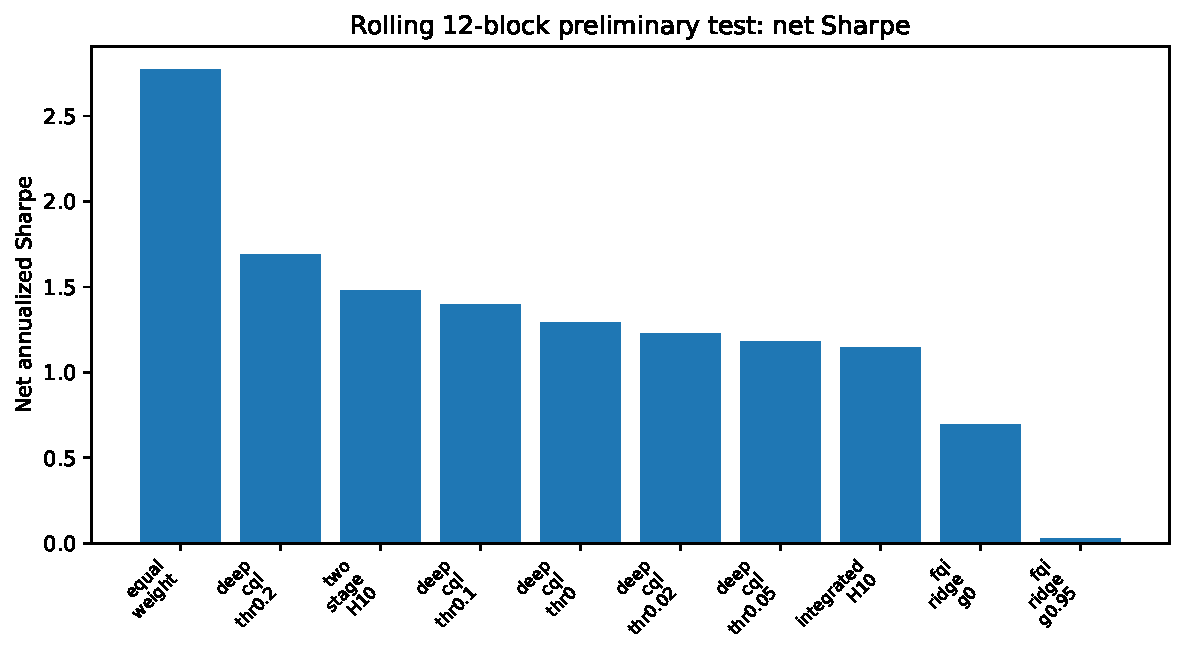
\includegraphics[width=0.90\linewidth]{figures/net_sharpe_bar.pdf}
\caption{Net annualized Sharpe across methods in the 12-roll preliminary test.}
\label{fig:net_sharpe}
\end{figure}

\begin{figure}[htbp]
\centering
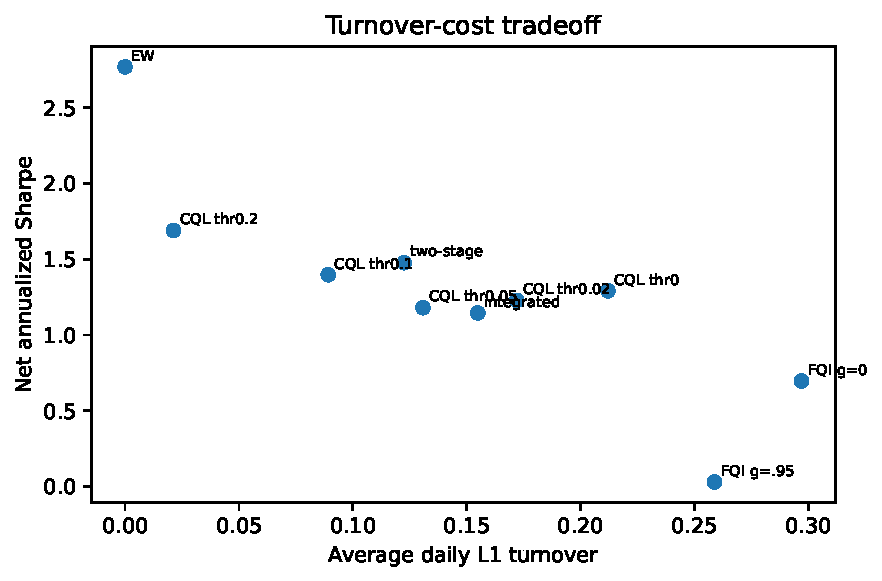
\includegraphics[width=0.75\linewidth]{figures/turnover_sharpe_scatter.pdf}
\caption{Average turnover versus net annualized Sharpe. High gross performance is insufficient if turnover is too large.}
\label{fig:turnover}
\end{figure}

\section{Discussion}

\paragraph{Why equal weight is hard to beat.}
The seven-ETF universe is broad and diversified. During the 2019 early rolling window used in the preliminary test, equities, bonds, gold, and credit-sensitive assets performed well. Equal weight therefore received diversified exposure with zero modeled turnover. This is a strong benchmark, not a trivial one. A learning strategy must generate enough active value to overcome both estimation error and transaction costs.

\paragraph{Why integrated learning did not help here.}
Integrated learning tries to align the prediction objective with the trading objective, but the empirical result suggests that this alignment is neither free nor guaranteed. The portfolio-level loss is noisy, the rolling training windows are short, and the optimizer-in-the-loop design is slow. In this implementation, the model appears to update before learning stable signals, and the resulting turnover is higher than in the two-stage baseline.

\paragraph{Why dynamic RL remains promising.}
The deep CQL-FQI proxy improves over plain FQI by combining three ideas: deep state representation, auxiliary prediction, and conservative/no-trade action selection. This supports the view that the decision layer should be dynamic and reward-aware. However, it also shows that the current alpha source is weak. The proposed direction should therefore be evaluated by active excess return over equal weight, not only by absolute NAV or Sharpe.

\paragraph{Reward design is the core research problem.}
The most important modeling choice is the reward:
\[
R_t =
w_t^\top r_{t+1}
-
c\|w_t-w_{t-1}\|_1
-
\eta w_t^\top \Sigma_t w_t
-
\rho\,\mathrm{DrawdownPenalty}_t.
\]
A poorly designed reward creates overtrading. A useful reward must trade off alpha, risk, transaction costs, drawdown, and the option value of not trading. Dynamic programming and RL are valuable because they allow these costs to be written directly as state-dependent future-value terms.

\section{Limitations}

This manuscript is preliminary and has several limitations:
\begin{enumerate}[leftmargin=*]
    \item The reported deep CQL-FQI test covers only 12 rolling blocks and 240 daily decisions.
    \item The universe has only seven ETFs; equal-weight diversification is unusually strong in this setting.
    \item The integrated method was not fully tuned over the large hyperparameter grids used in more complete studies.
    \item The deep RL method uses a finite candidate action set, not a continuous action space.
    \item The equal-weight baseline is modeled with zero turnover; a fairer future study should include daily rebalanced equal weight and buy-and-hold equal weight separately.
    \item The data are proprietary Wind data accessed through Boke City / Boke Simu; public replication requires a public data replacement.
\end{enumerate}

\section{Future Work}

The final research goal is a constrained dynamic prediction-decision architecture for portfolio optimization. Future work will:
\begin{enumerate}[leftmargin=*]
    \item extend the rolling test to the full 2019--2024 out-of-sample period;
    \item evaluate active excess returns over equal weight and not only absolute portfolio returns;
    \item add regime and macro features, including volatility, rates, and cross-asset correlation states;
    \item replace the simple MLP encoder with TCN, CNN-LSTM, or PatchTST-style encoders;
    \item test conservative Q-learning, implicit Q-learning, and TD3+BC for continuous action spaces;
    \item tune reward coefficients for transaction cost, variance, drawdown, and no-trade thresholds;
    \item compare two-stage, integrated, and dynamic RL methods under the same validation protocol.
\end{enumerate}

\section{Conclusion}

This preliminary study investigates whether dynamic portfolio optimization should be approached through integrated prediction-optimization or through a modular prediction-decision architecture. The experiments do not support a direct shift from two-stage learning to integrated learning in the tested seven-ETF setting: two-stage is faster and performs better out of sample. Plain FQI is also insufficient because it overtrades. A deep conservative FQI decision layer is more promising: it combines deep prediction with Bellman value learning and no-trade constraints, and it improves over the learned baselines in the preliminary rolling test. Nevertheless, equal weight remains strongest, showing that the current method has not yet discovered robust active alpha.

The main contribution of this draft is therefore conceptual and diagnostic. Portfolio optimization is dynamic because current holdings affect future costs and opportunities. Deep learning can model the past-to-future market state, while reinforcement learning can model the current-action-to-future-value relationship. The practical challenge is not merely to integrate prediction and optimization, but to design a reward and policy class that learns dynamic value without overtrading in scarce, noisy financial data.

\section*{Acknowledgments}

This work was initiated during the author's internship at Boke Simu. The ETF data used in the preliminary experiments were sourced from Wind data accessed through Boke City / Boke Simu. The views expressed in this preliminary draft are those of the author and do not necessarily represent Boke Simu or Columbia University.

\section*{Data and Code Availability}

The raw data are not redistributed because they were obtained from proprietary Wind data access. The experimental scripts are designed to accept a public replacement ETF price panel in the same format. A public replication package should replace the proprietary data with public ETF prices and re-run the rolling experiments.

\section*{Disclaimer}

This manuscript is for academic research only and is not investment advice. The preliminary results should not be used to make trading or investment decisions.

\bibliographystyle{plainnat}
\bibliography{references}

\end{document}
